%!TEX root = ../thesis-guntur.tex
%********************************************************************
% Appendix
%*******************************************************
% If problems with the headers: get headings in appendix etc. right
%\markboth{\spacedlowsmallcaps{Appendix}}{\spacedlowsmallcaps{Appendix}}
\chapter{Access Point Count Correlation}
\label{ch:appendix-sensor-readings}

\section{Scatter Plots} % (fold)
\label{sec:scatter-plots}
% ap vs head count
\begin{figure}[H]
  \begin{adjustwidth}{-1cm}{}
  \centering
  \subfloat[day 1]{
    \label{fig:ap-hc-day1}{
      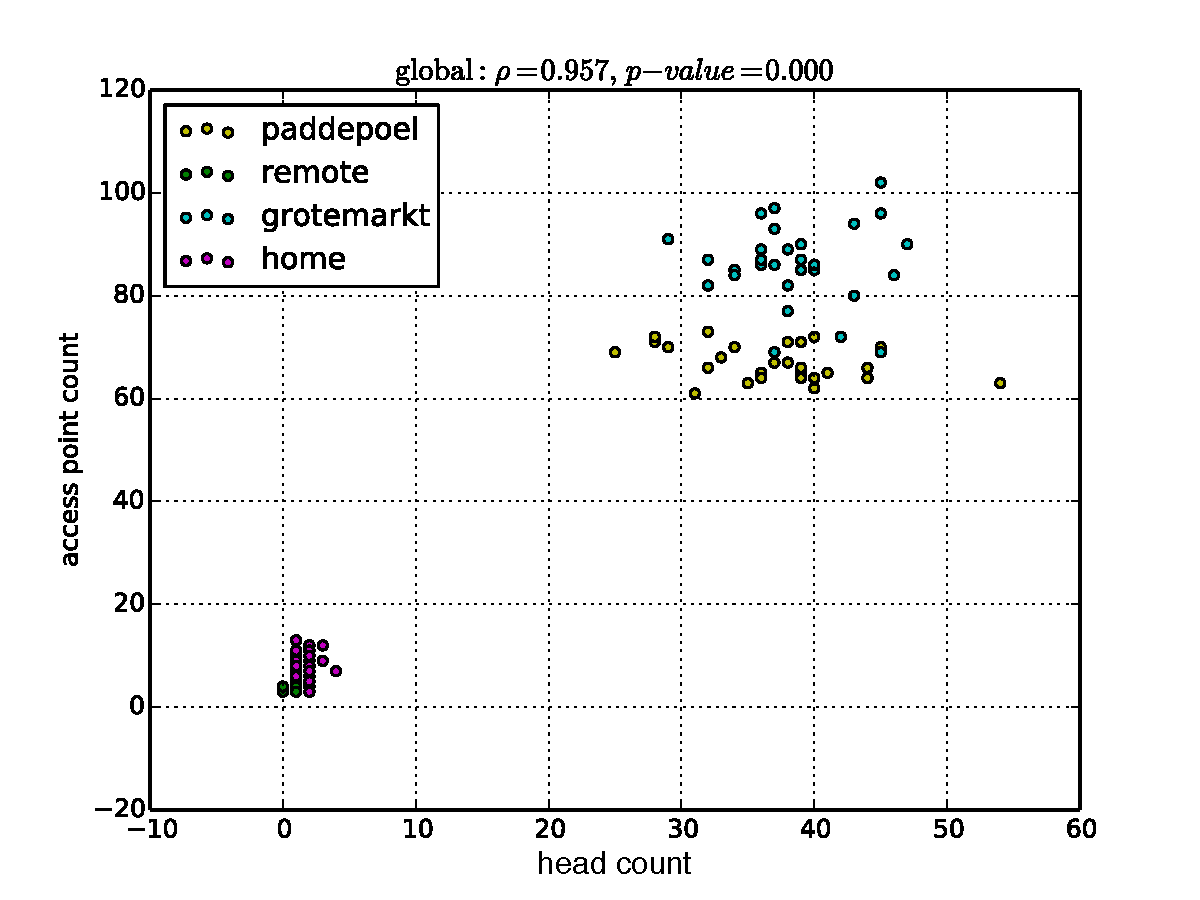
\includegraphics[width=0.7\textwidth]{./img/result/day/day1/global-gt-vs-ap}
    }
  }
  \subfloat[day 2]{
    \label{fig:ap-hc-day2}{
      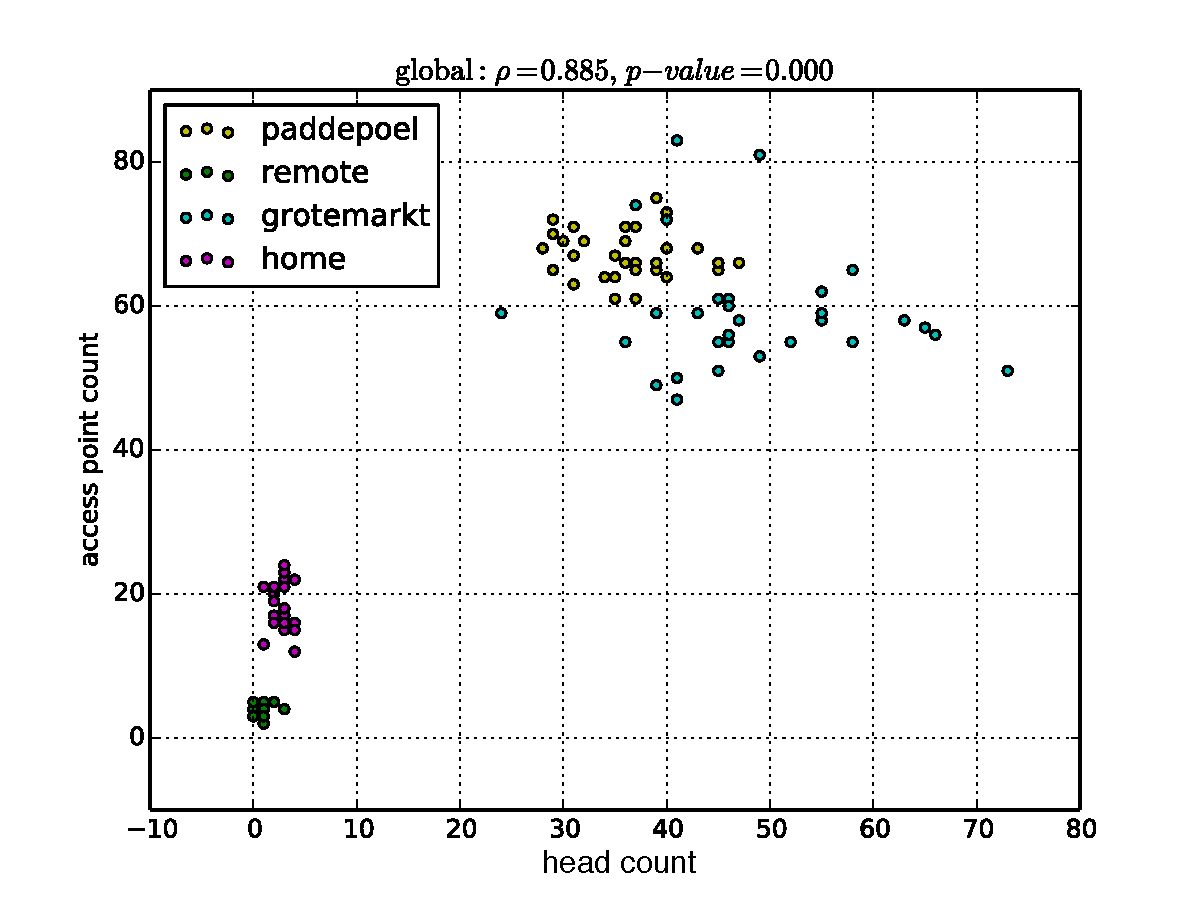
\includegraphics[width=0.7\textwidth]{./img/result/day/day2/global-gt-vs-ap}
    }
  }\\
  \subfloat[day 3]{
    \label{fig:ap-hc-day3}{
      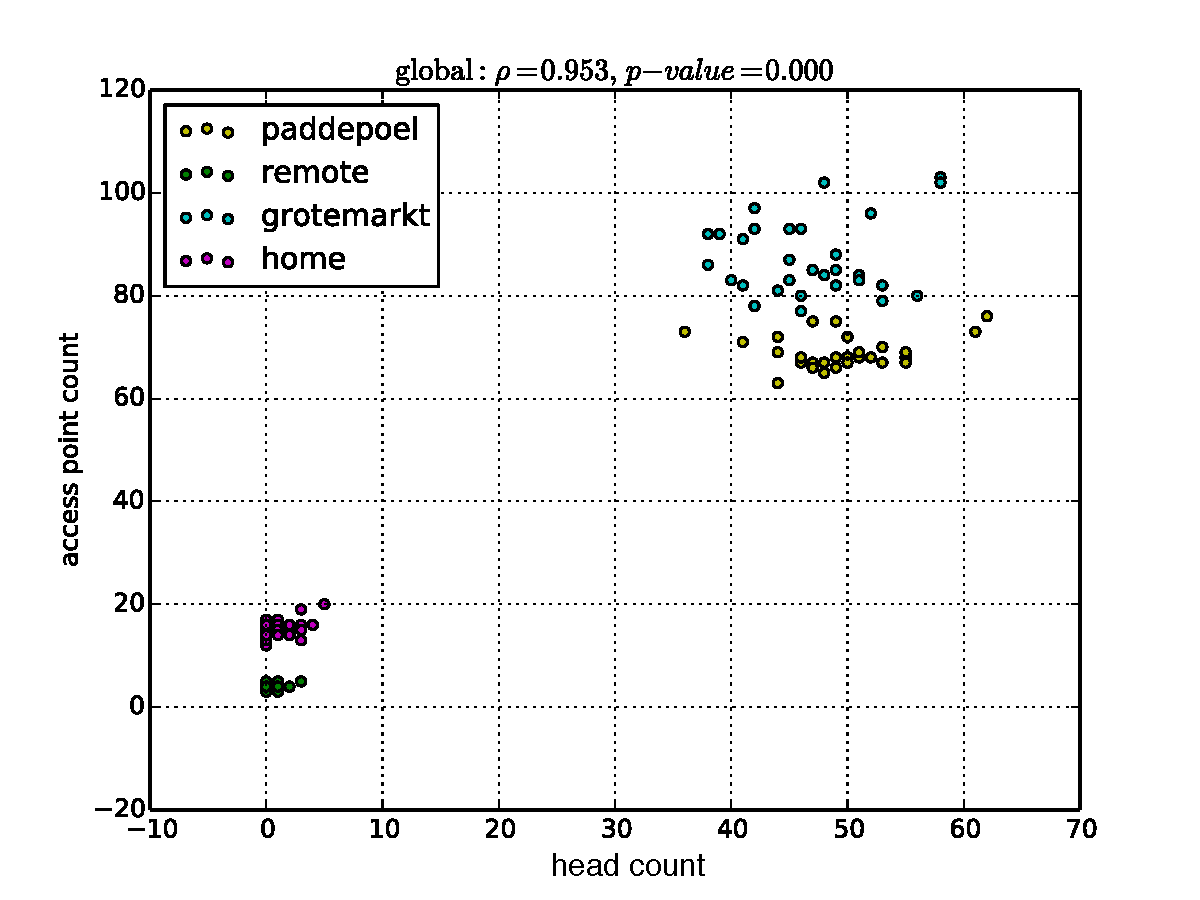
\includegraphics[width=0.7\textwidth]{./img/result/day/day3/global-gt-vs-ap}
    }
  }
  \subfloat[day 4]{
    \label{fig:ap-hc-day4}{
      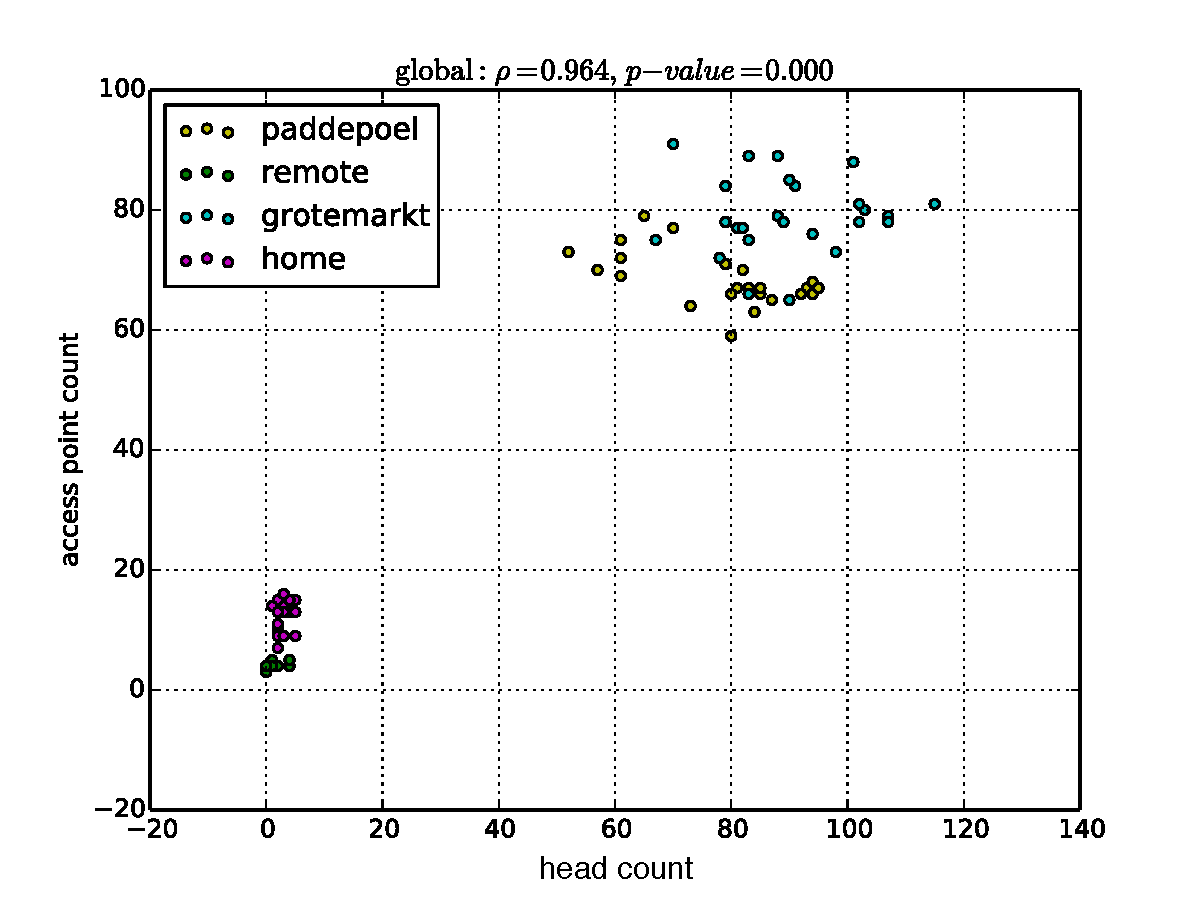
\includegraphics[width=0.7\textwidth]{./img/result/day/day4/global-gt-vs-ap}
    }
  }
  \end{adjustwidth}
  \caption[The scatter plots of the correlation between headcount and \ac{AP} count.]
  {The scatter plots showing the correlation between headcount and \ac{AP} count in four days of experiment. The location is coded in color.}
  \label{fig:ap-hc-scatterplot}
\end{figure}

% ap vs device count
\begin{figure}[H]
  \begin{adjustwidth}{-3cm}{}
  \centering
  \subfloat[day 1]{
    \label{fig:ap-dc-day1}{
      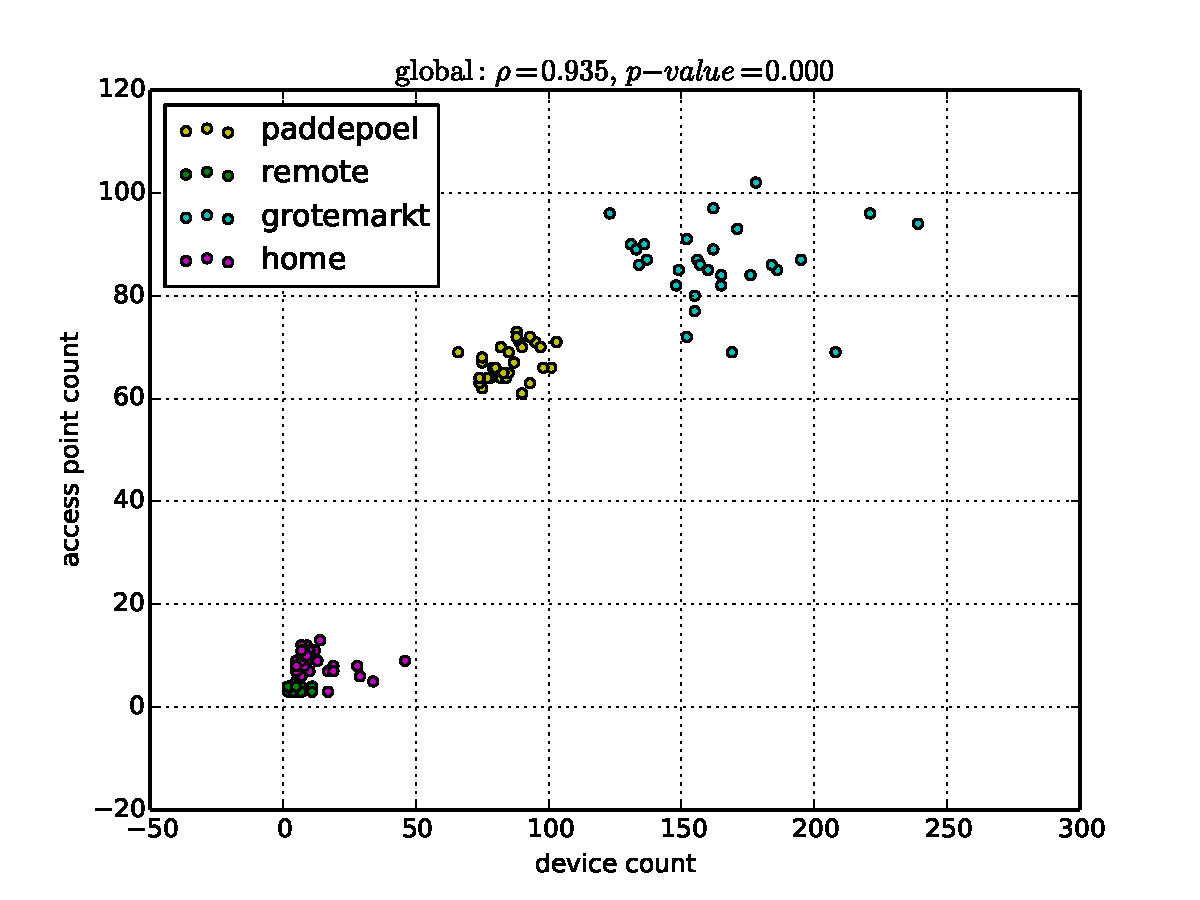
\includegraphics[width=0.7\textwidth]{./img/result/day/day1/global-pr-vs-ap}
    }
  }
  \subfloat[day 2]{
    \label{fig:ap-dc-day2}{
      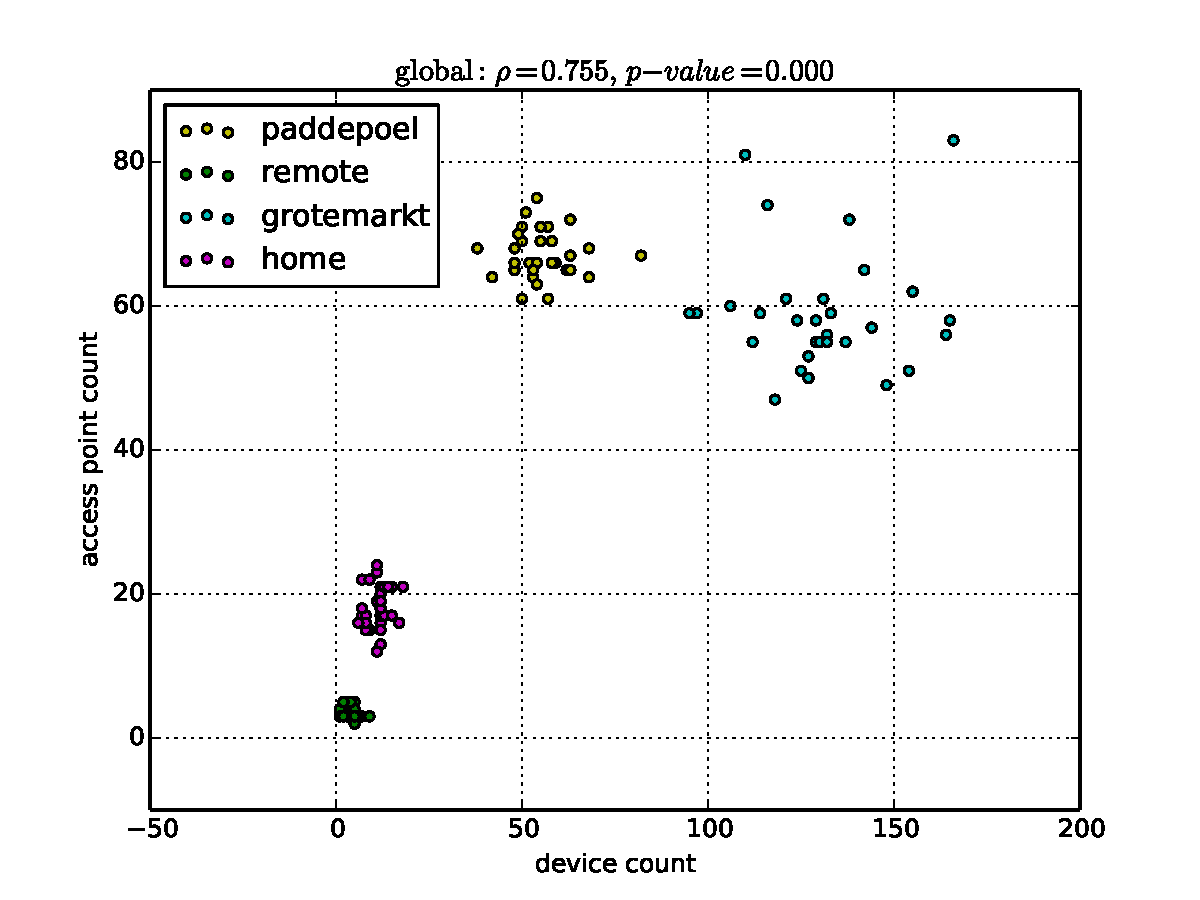
\includegraphics[width=0.7\textwidth]{./img/result/day/day2/global-pr-vs-ap}
    }
  }\\
  \subfloat[day 3]{
    \label{fig:ap-dc-day3}{
      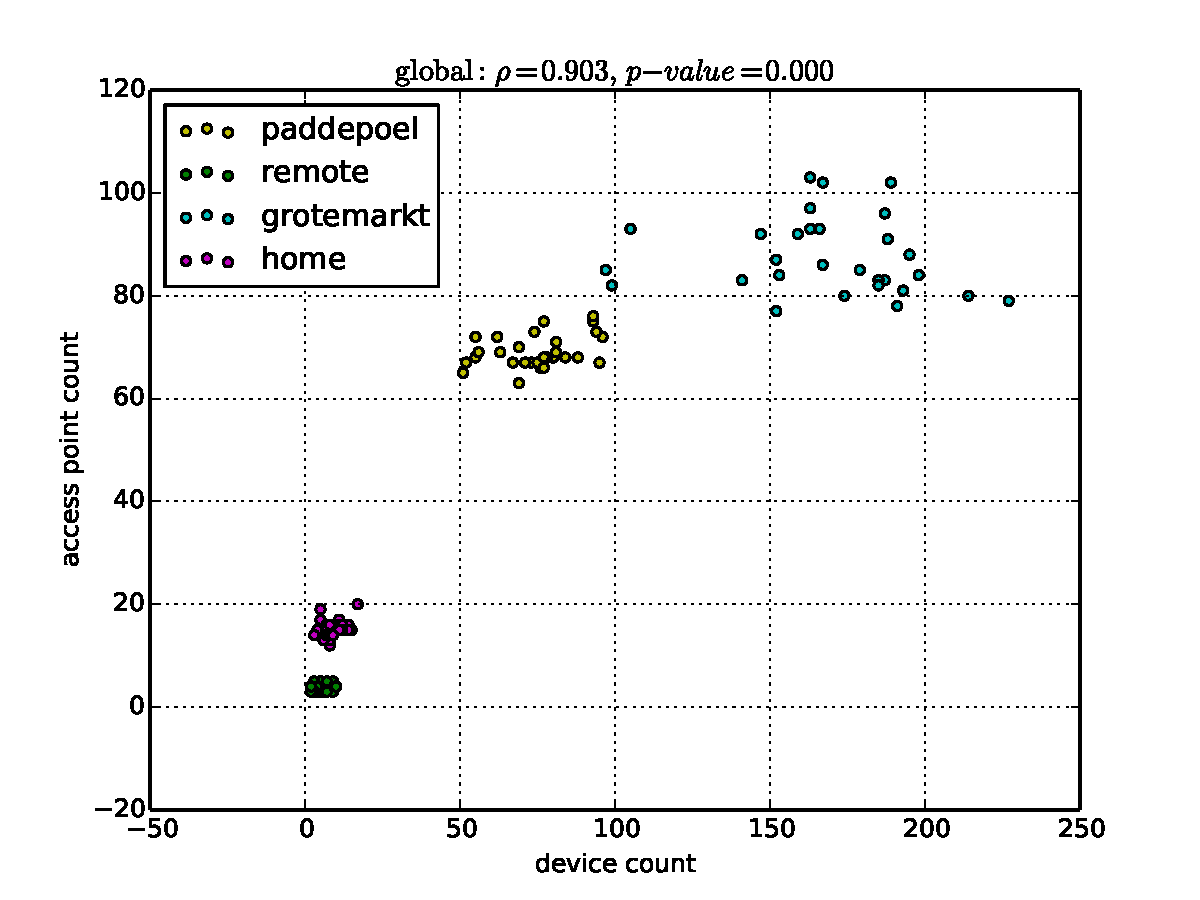
\includegraphics[width=0.7\textwidth]{./img/result/day/day3/global-pr-vs-ap}
    }
  }
  \subfloat[day 4]{
    \label{fig:ap-dc-day4}{
      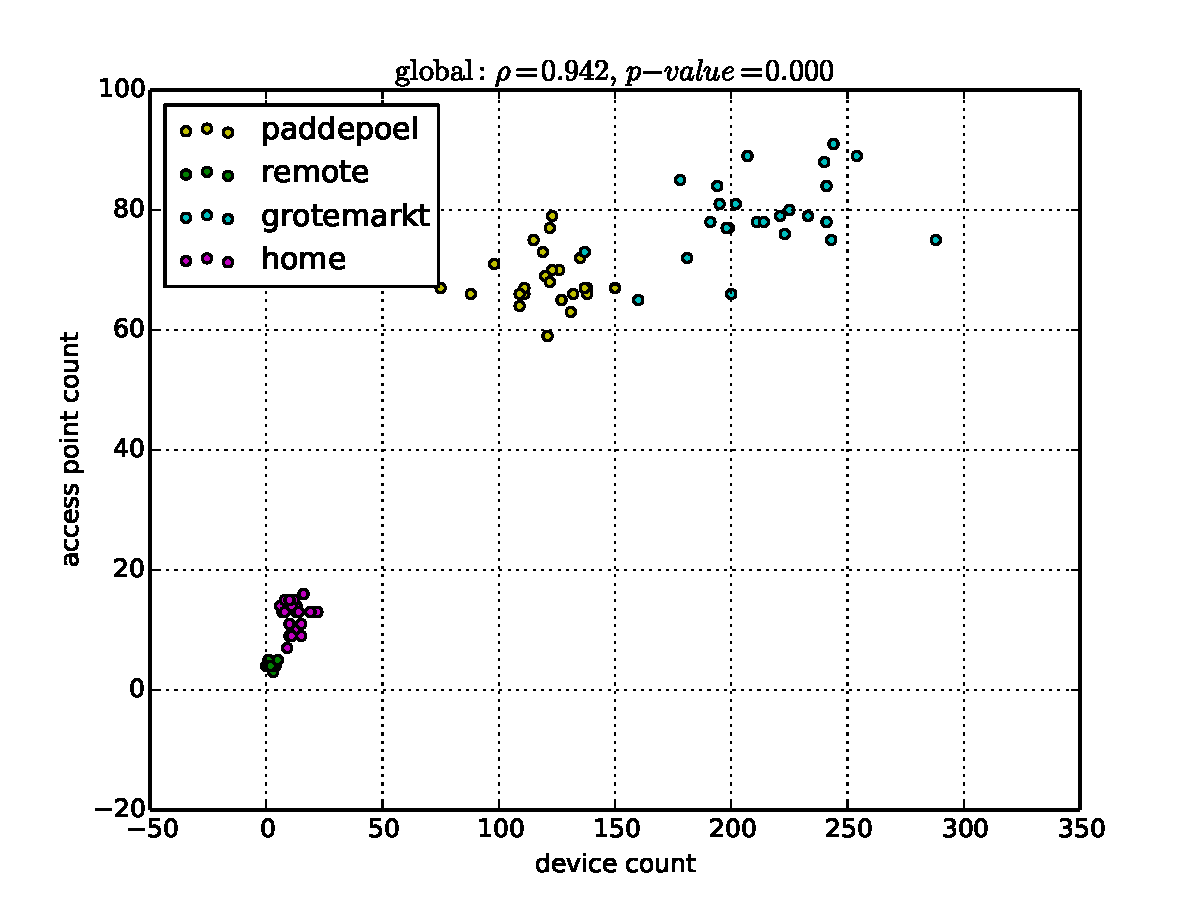
\includegraphics[width=0.7\textwidth]{./img/result/day/day4/global-pr-vs-ap}
    }
  }
  \end{adjustwidth}
  \caption[The scatter plots of the correlation between device count and \ac{AP}.]
  {The scatter plots showing the correlation between device count and \ac{AP} count in four days of experiment. The location is coded in color.}
  \label{fig:ap-dc-scatterplot}
\end{figure}

% ap vs device count
\begin{figure}[H]
  \begin{adjustwidth}{-1cm}{}
  \centering
  \subfloat[day 1]{
    \label{fig:hc-dc-day1}{
      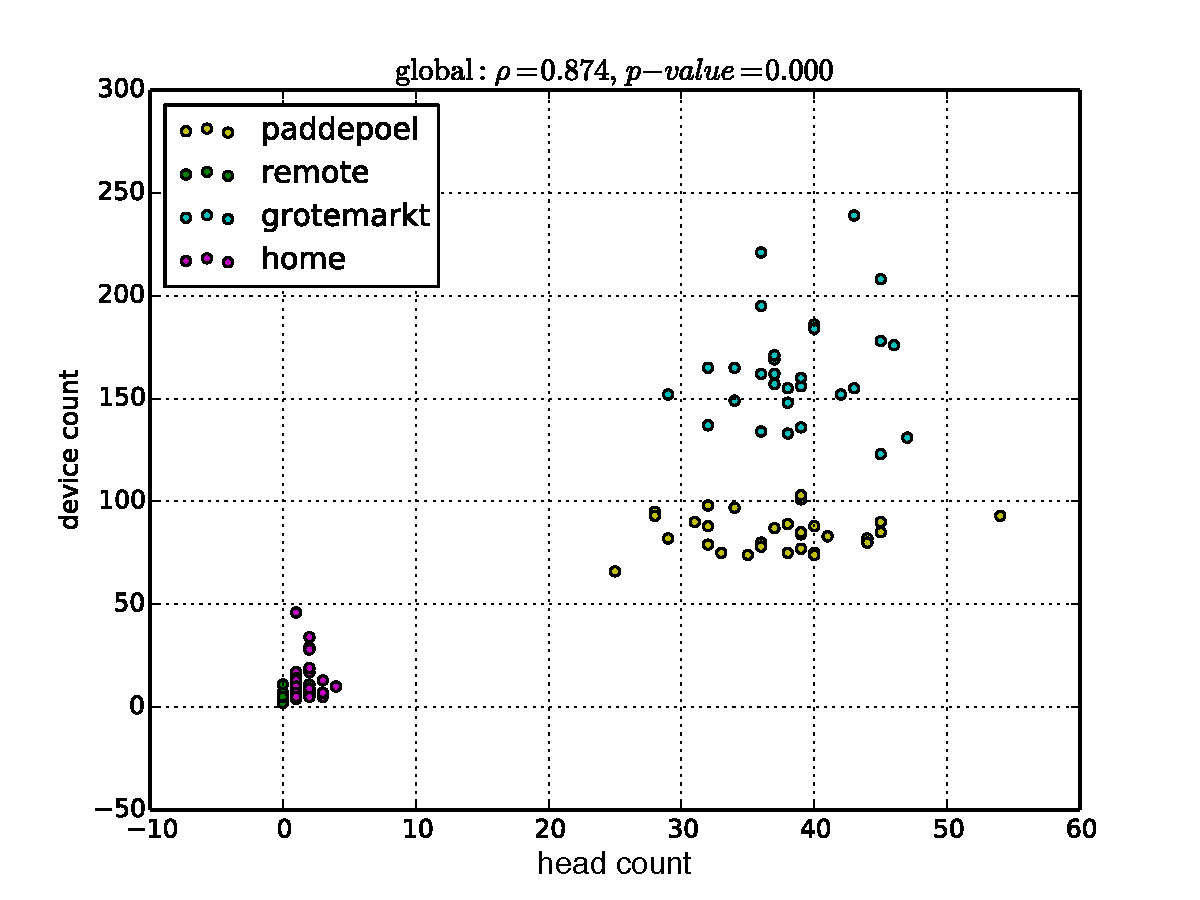
\includegraphics[width=0.7\textwidth]{./img/result/day/day1/global-gt-vs-pr}
    }
  }
  \subfloat[day 2]{
    \label{fig:hc-dc-day2}{
      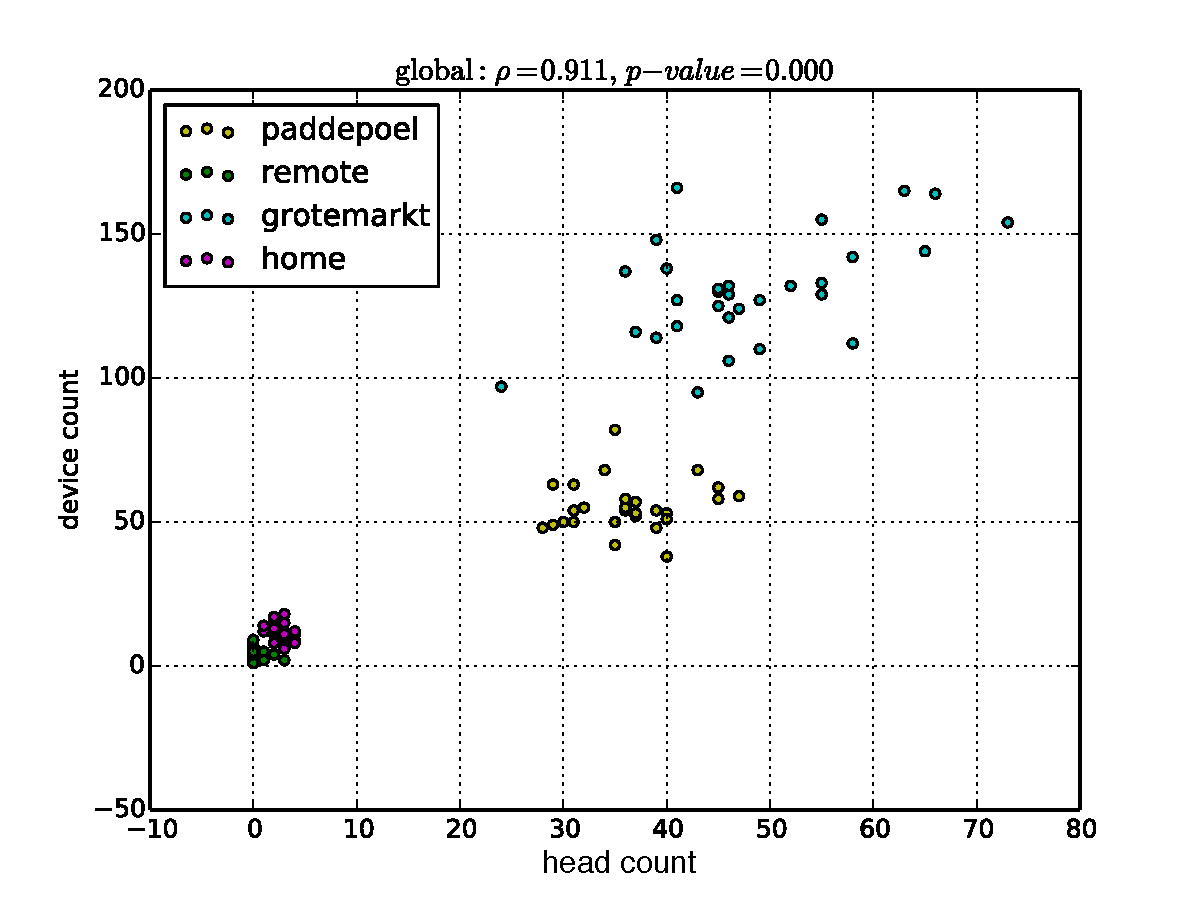
\includegraphics[width=0.7\textwidth]{./img/result/day/day2/global-gt-vs-pr}
    }
  }\\
  \subfloat[day 3]{
    \label{fig:hc-dc-day3}{
      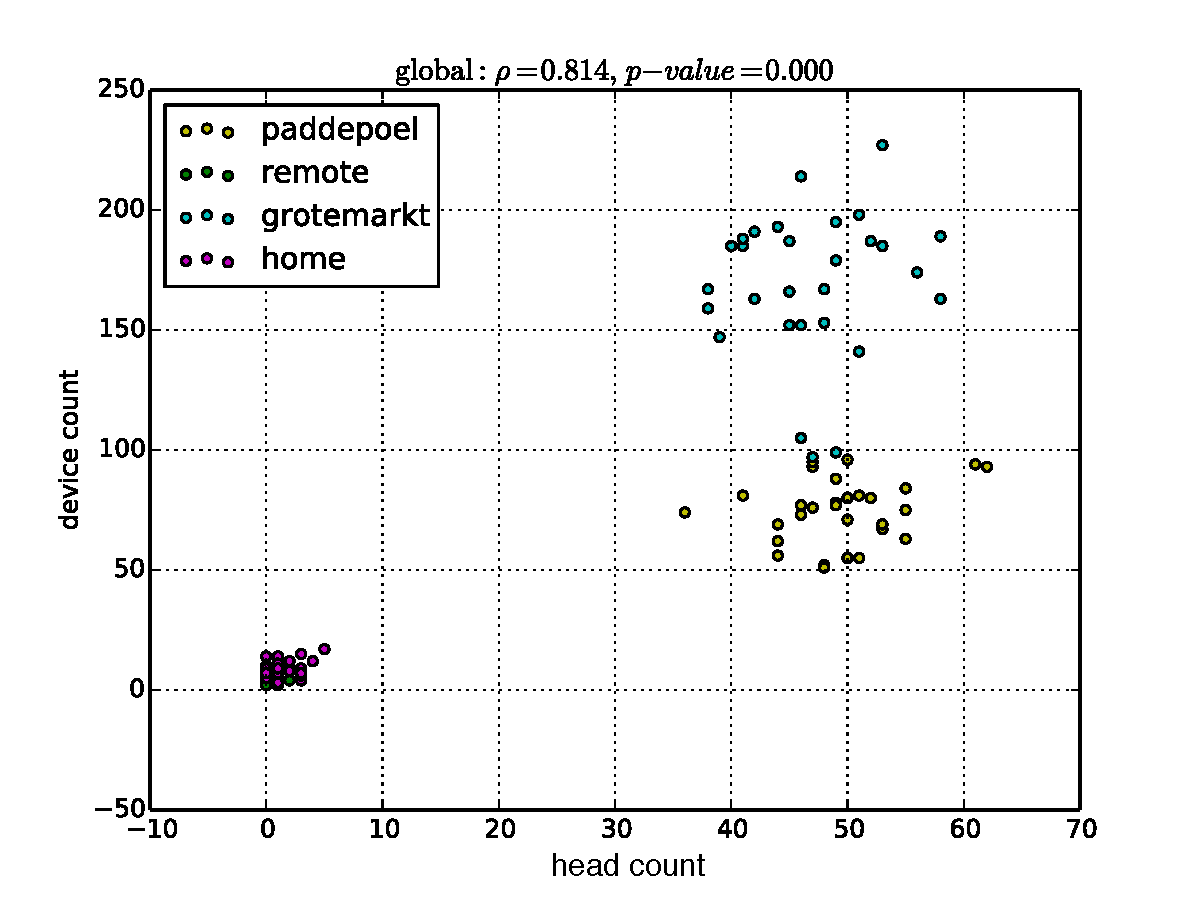
\includegraphics[width=0.7\textwidth]{./img/result/day/day3/global-gt-vs-pr}
    }
  }
  \subfloat[day 4]{
    \label{fig:hc-dc-day4}{
      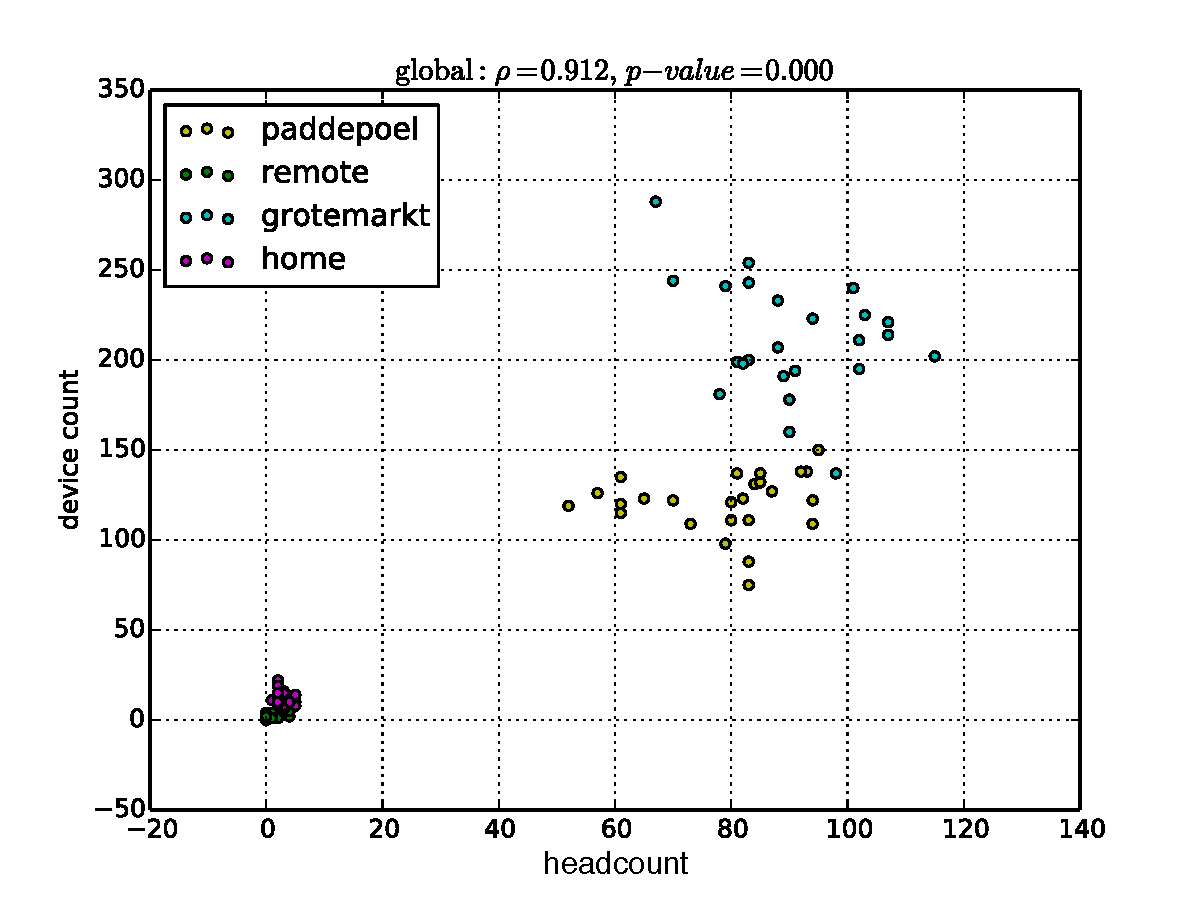
\includegraphics[width=0.7\textwidth]{./img/result/day/day4/global-gt-vs-pr}
    }
  }
  \end{adjustwidth}
  \caption[The scatter plots of the correlation between device count and \ac{AP} count.]
  {The scatter plots showing the correlation between device count and \ac{AP} count in four days of experiment. The location is coded in color.}
  \label{fig:hc-dc-scatterplot}
\end{figure}







\section{Line charts} % (fold)
\label{sec:line_charts}

\begin{figure}[H]
  \begin{adjustwidth}{-5cm}{}
  \centering
  \subfloat[day 1]{
    \label{fig:remote-day1}{
      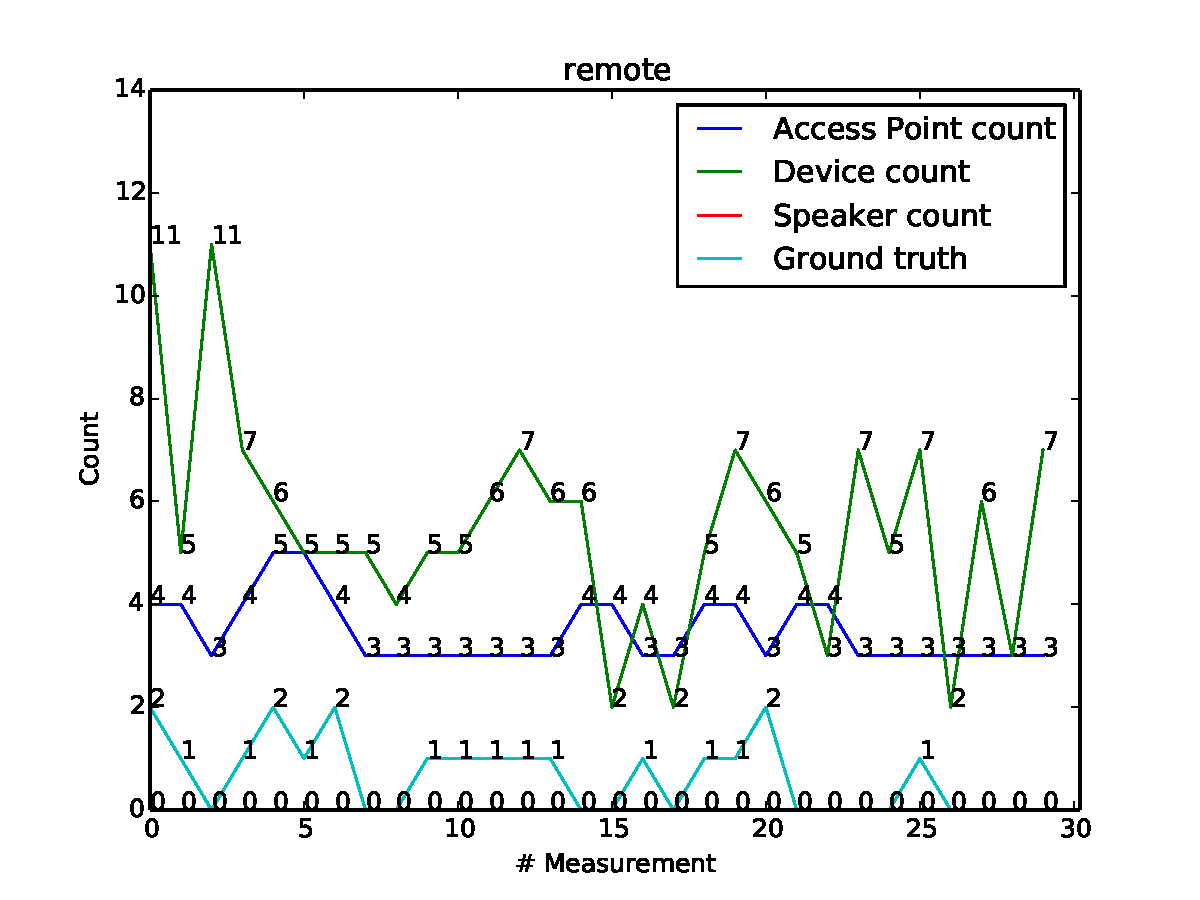
\includegraphics[width=0.7\textwidth]{./img/result/day/day1/remote-20161026}
    }
  }
  \subfloat[day 2]{
    \label{fig:remote-day2}{
      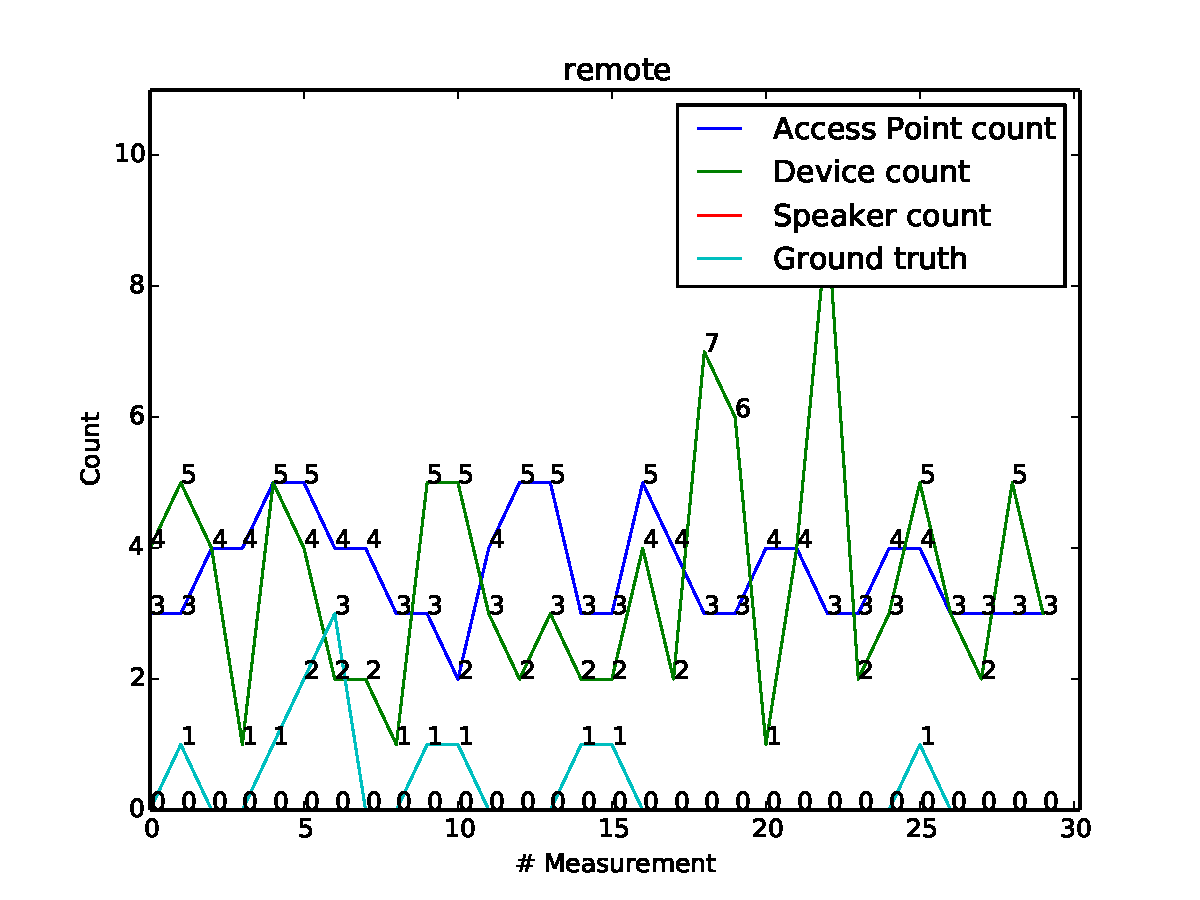
\includegraphics[width=0.7\textwidth]{./img/result/day/day2/remote-20161027}
    }
  }\\
  \subfloat[day 3]{
    \label{fig:remote-day3}{
      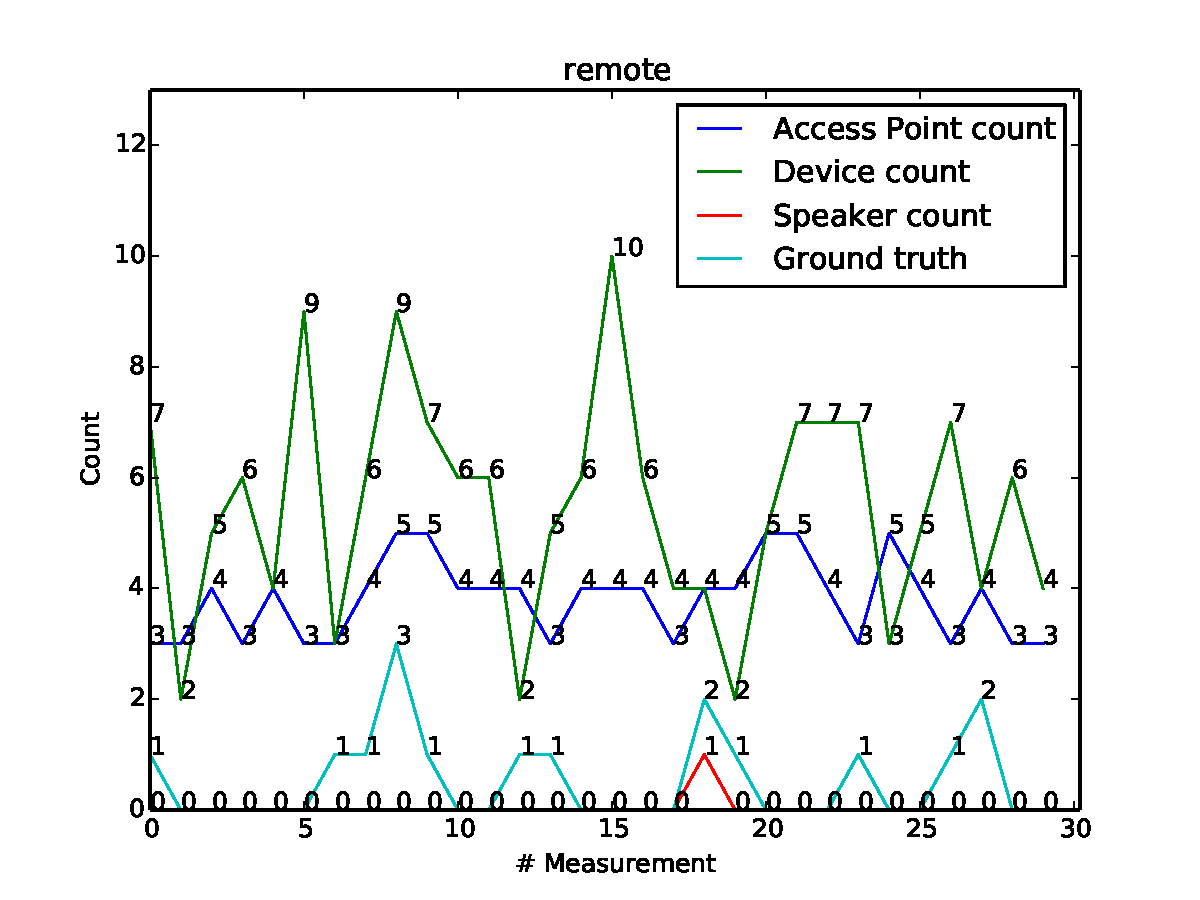
\includegraphics[width=0.7\textwidth]{./img/result/day/day3/remote-20161028}
    }
  }
  \subfloat[day 4]{
    \label{fig:remote-day4}{
      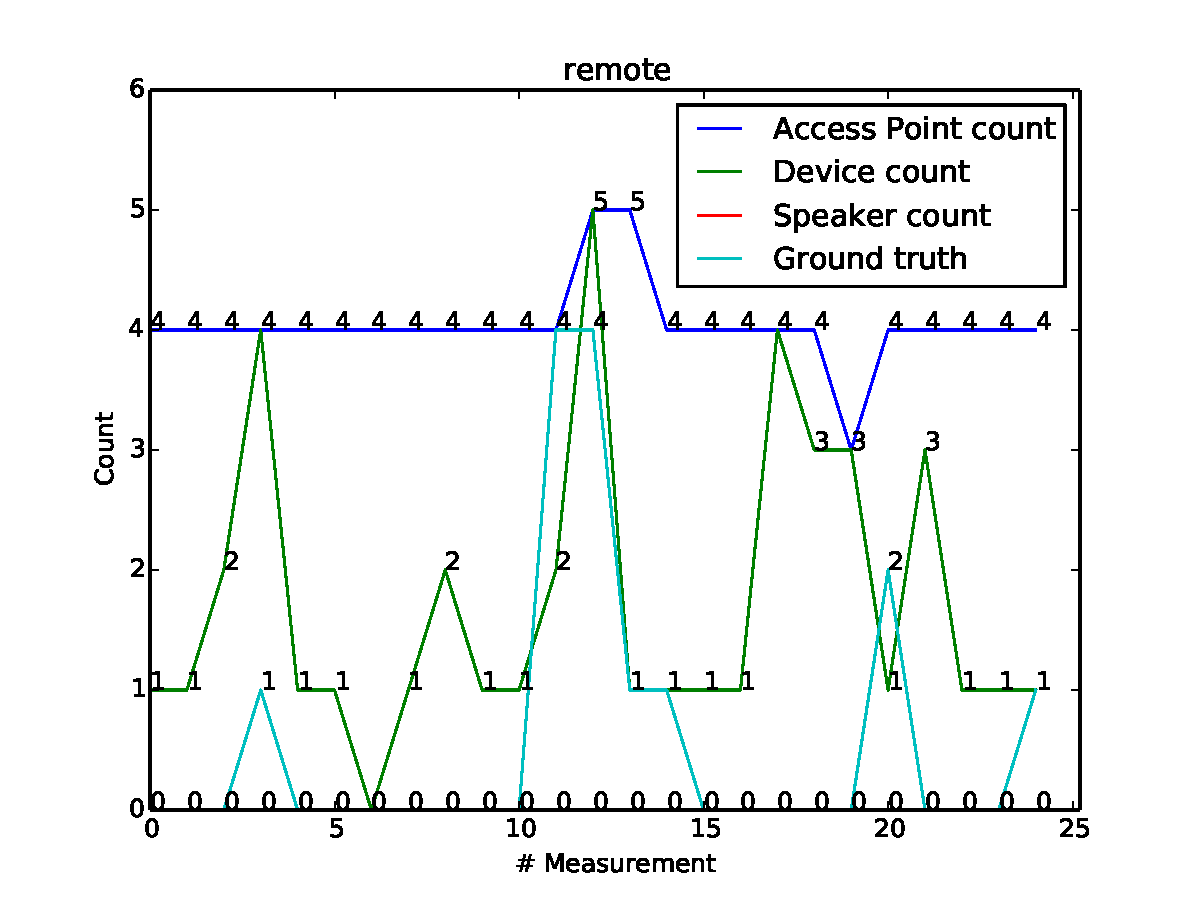
\includegraphics[width=0.7\textwidth]{./img/result/day/day4/remote-20161029}
    }
  }
  \end{adjustwidth}
  \caption[The line chart of sensor readings at remote area.]
  {The line chart of sensor readings at \textit{remote area} in four days of experiment.}
  \label{fig:result-remote-line-chart}
\end{figure}


\begin{figure}[H]
  \begin{adjustwidth}{-1cm}{}
  \centering
  \subfloat[day 1]{
    \label{fig:home-day1}{
      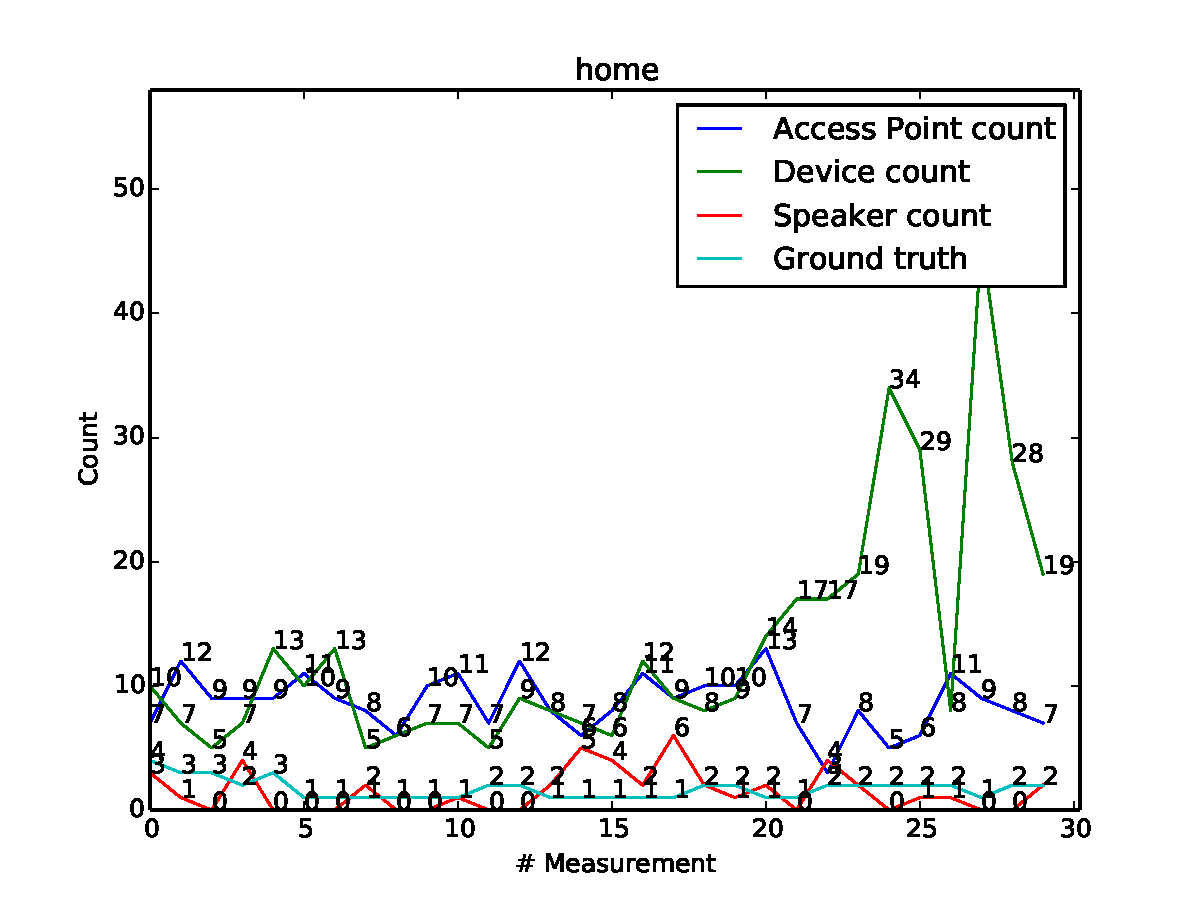
\includegraphics[width=0.7\textwidth]{./img/result/day/day1/home-20161026}
    }
  }
  \subfloat[day 2]{
    \label{fig:home-day2}{
      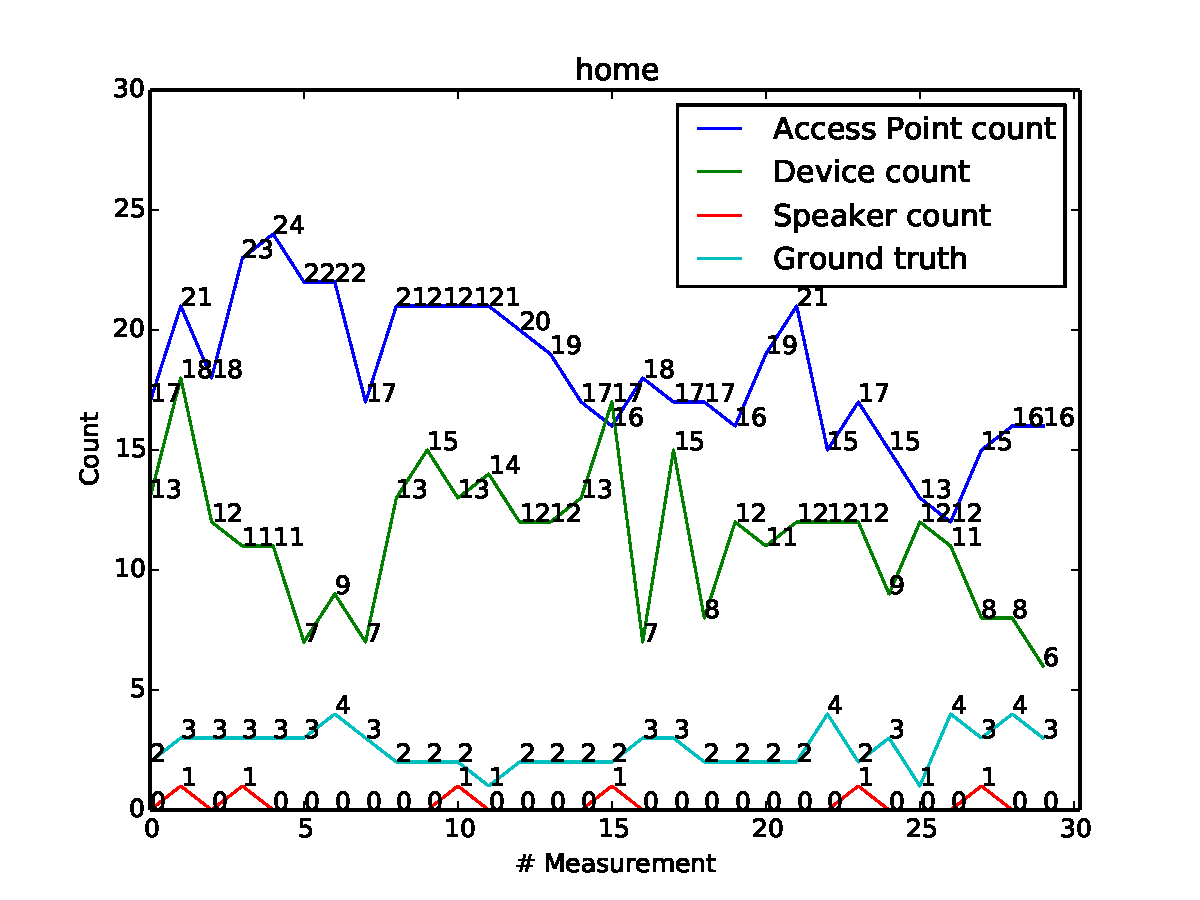
\includegraphics[width=0.7\textwidth]{./img/result/day/day2/home-20161027}
    }
  }\\
  \subfloat[day 3]{
    \label{fig:home-day3}{
      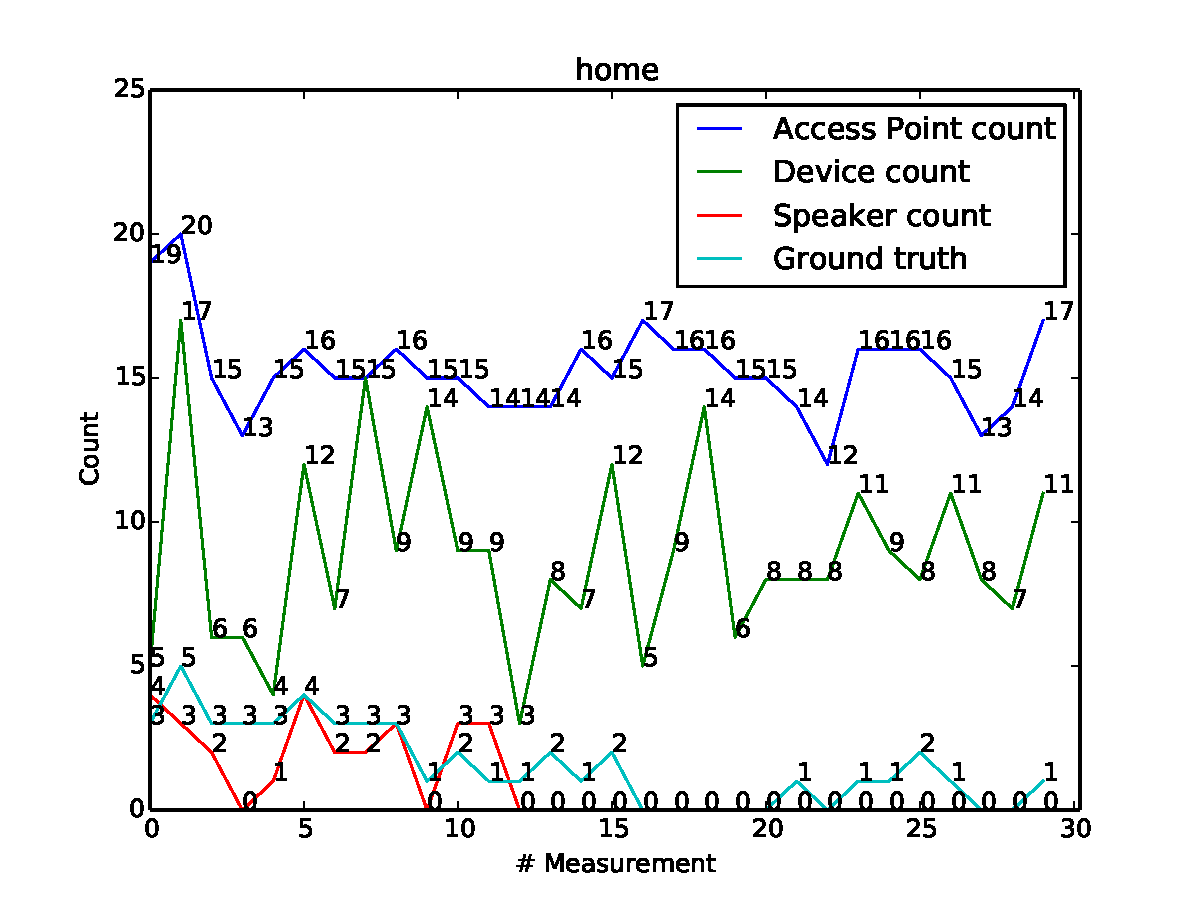
\includegraphics[width=0.7\textwidth]{./img/result/day/day3/home-20161028}
    }
  }
  \subfloat[day 4]{
    \label{fig:home-day4}{
      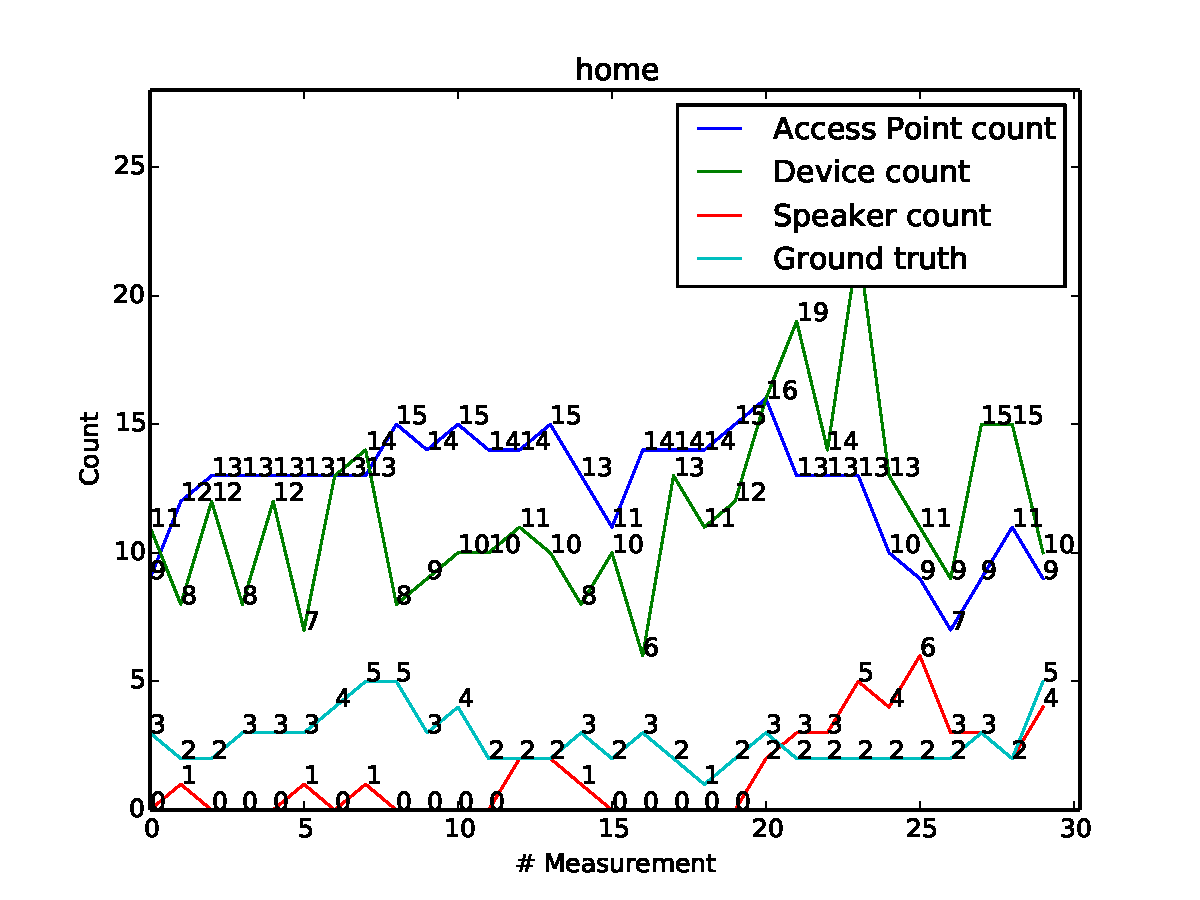
\includegraphics[width=0.7\textwidth]{./img/result/day/day4/home-20161029}
    }
  }
  \end{adjustwidth}
  \caption[The line chart of sensor readings at home.]
  {The line chart of sensor readings at \textit{home} in four days of experiment.}
  \label{fig:result-home-line-chart}
\end{figure}


\begin{figure}[H]
  \begin{adjustwidth}{-5cm}{}
  \centering
  \subfloat[day 1]{
    \label{fig:paddepoel-day1}{
      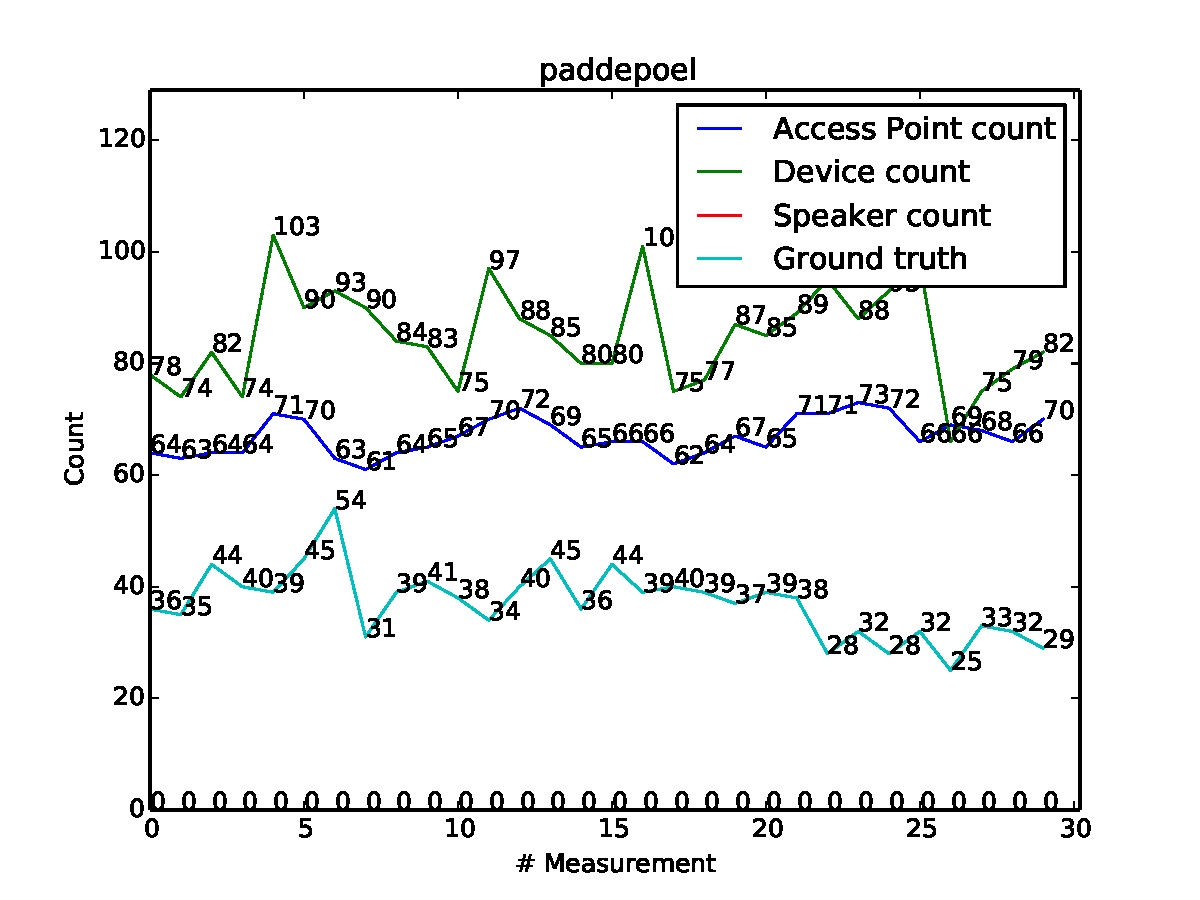
\includegraphics[width=0.7\textwidth]{./img/result/day/day1/paddepoel-20161026}
    }
  }
  \subfloat[day 2]{
    \label{fig:paddepoel-day2}{
      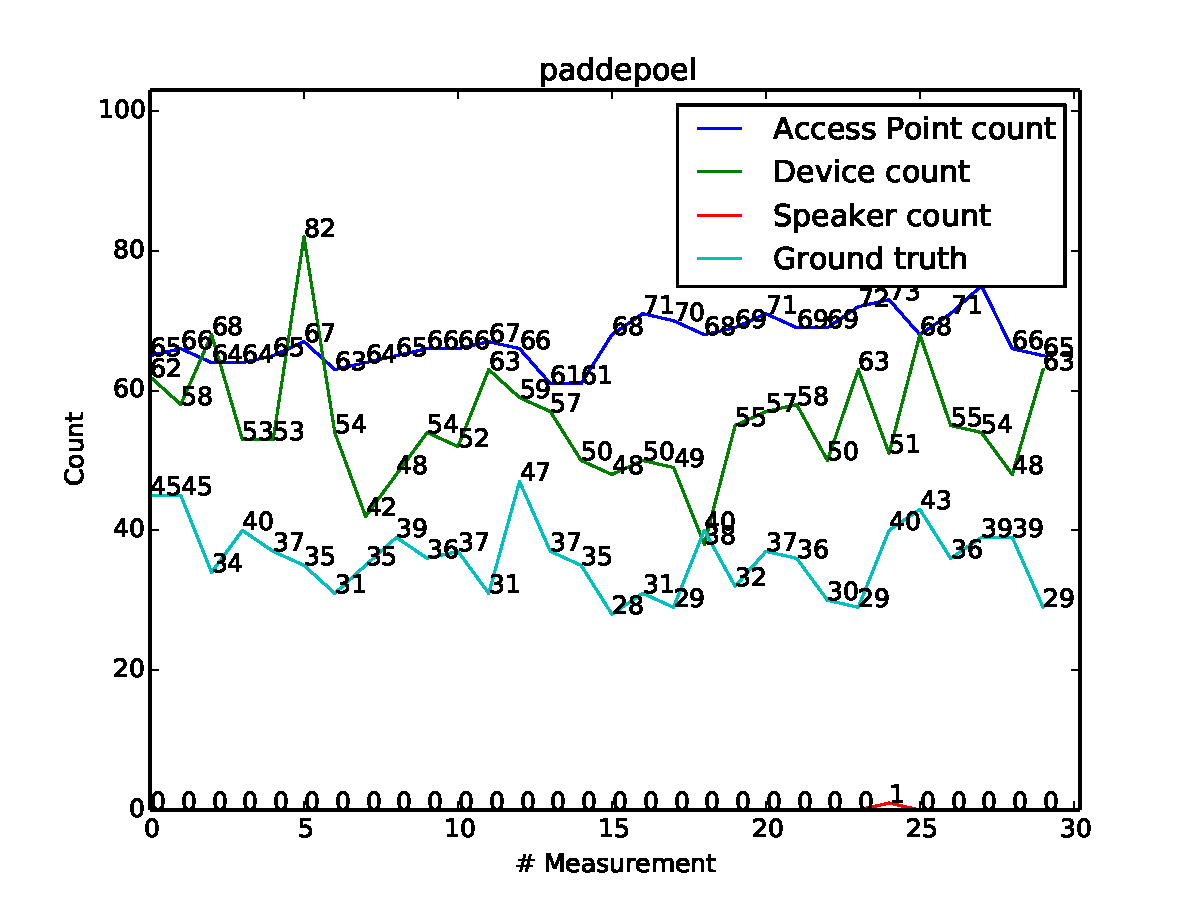
\includegraphics[width=0.7\textwidth]{./img/result/day/day2/paddepoel-20161027}
    }
  }\\
  \subfloat[day 3]{
    \label{fig:paddepoel-day3}{
      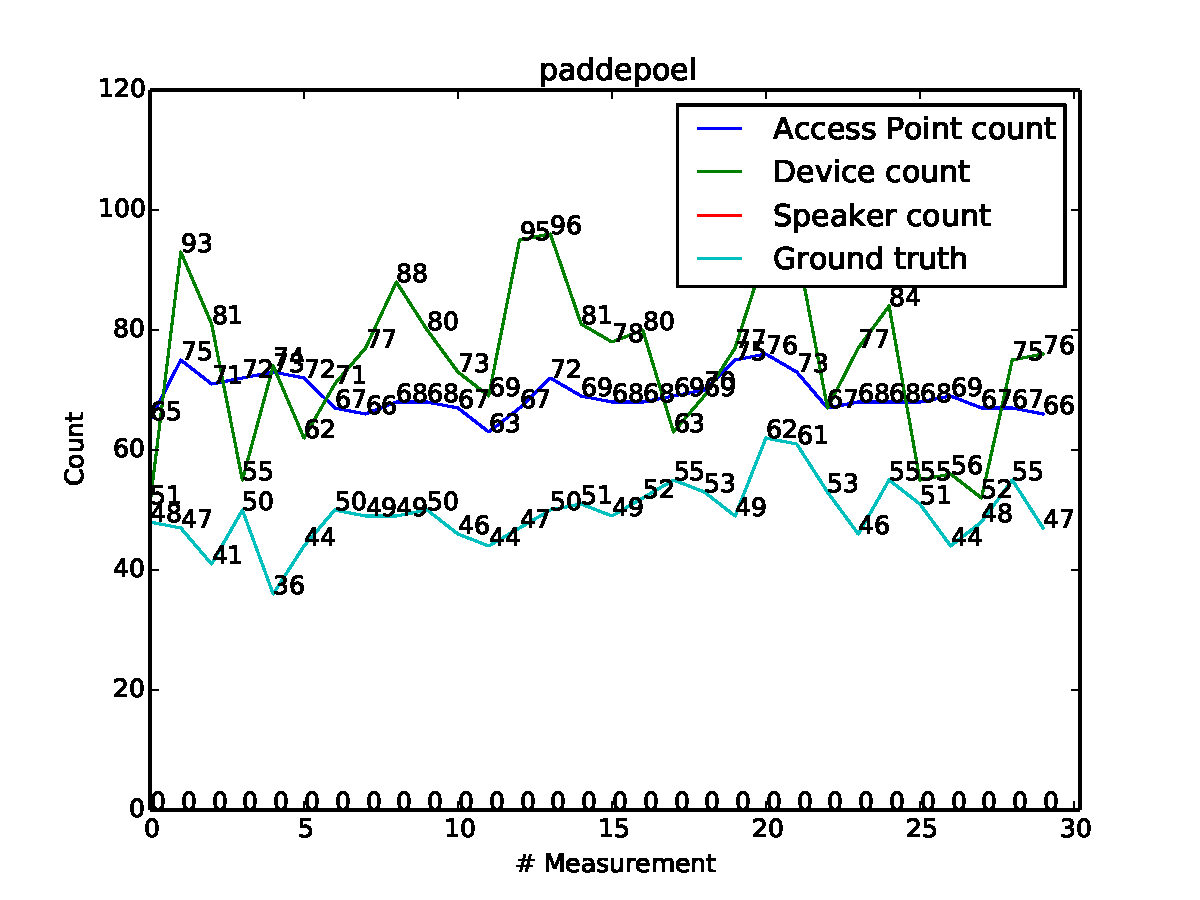
\includegraphics[width=0.7\textwidth]{./img/result/day/day3/paddepoel-20161028}
    }
  }
  \subfloat[day 4]{
    \label{fig:paddepoel-day4}{
      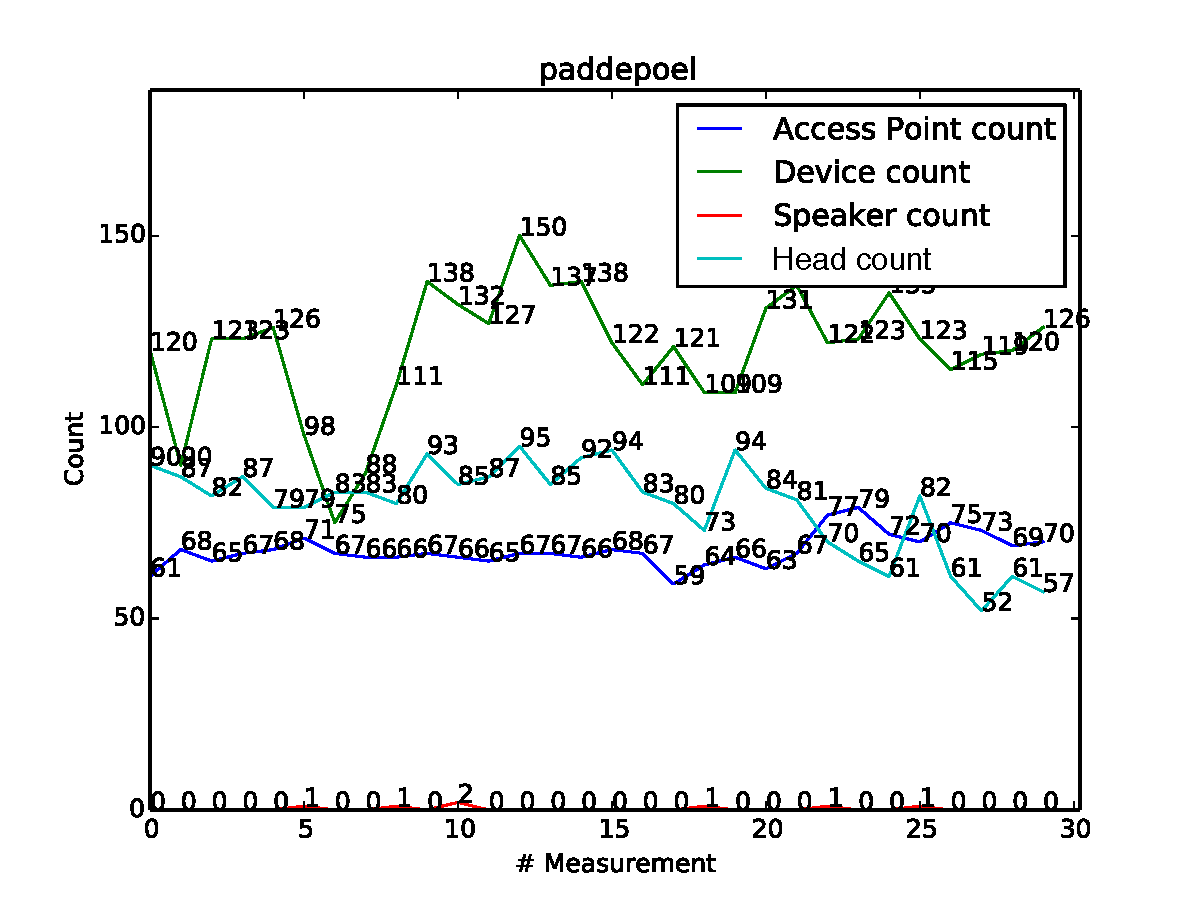
\includegraphics[width=0.7\textwidth]{./img/result/day/day4/paddepoel-20161029}
    }
  }
  \end{adjustwidth}
  \caption[The line chart of sensor readings at Paddepoel Shopping Center.]
  {The line chart of sensor readings at \textit{Paddepoel Shopping Center} in four days of experiment.}
  \label{fig:result-paddepoel-line-chart}
\end{figure}


\begin{figure}[H]
  \begin{adjustwidth}{-2cm}{}
  \centering
  \subfloat[day 1]{
    \label{fig:grotemarkt-day1}{
      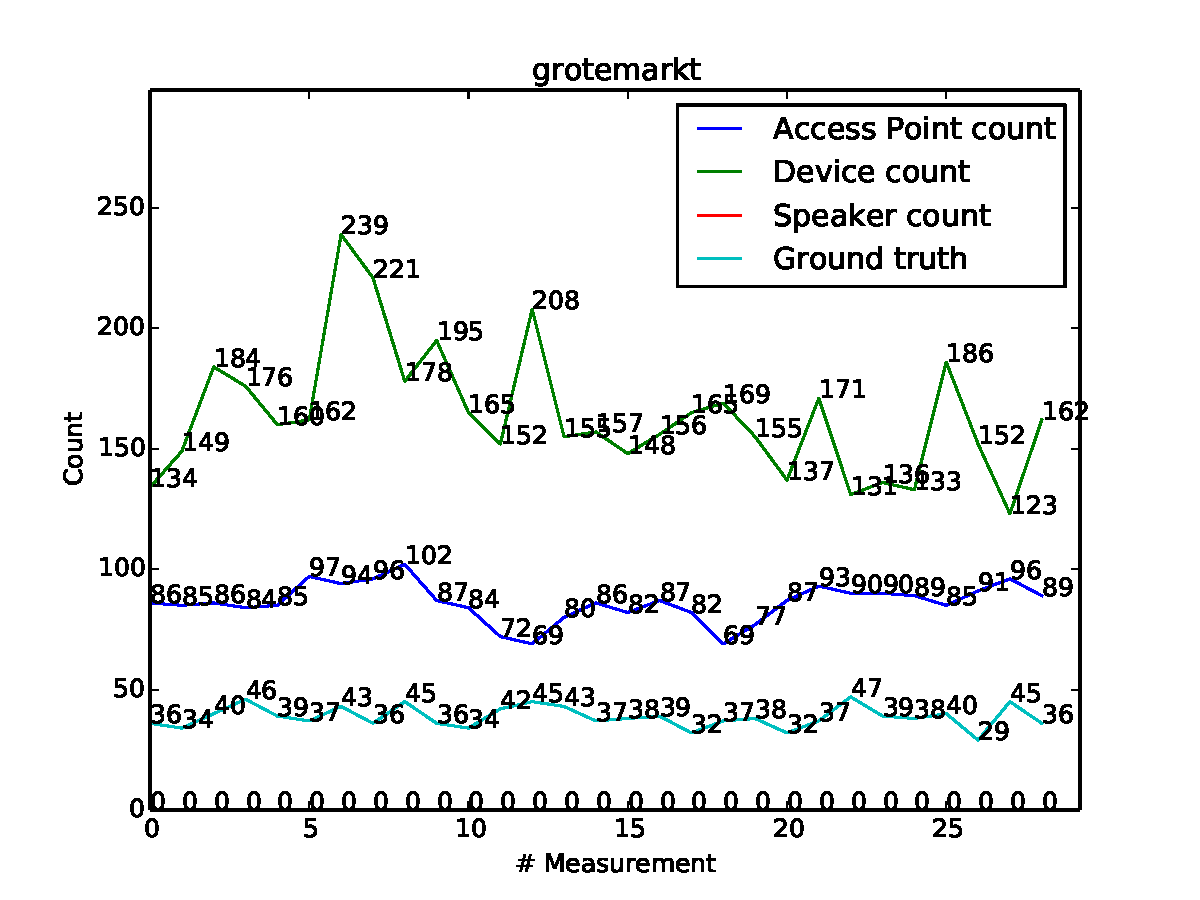
\includegraphics[width=0.7\textwidth]{./img/result/day/day1/grotemarkt-20161026}
    }
  }
  \subfloat[day 2]{
    \label{fig:grotemarkt-day2}{
      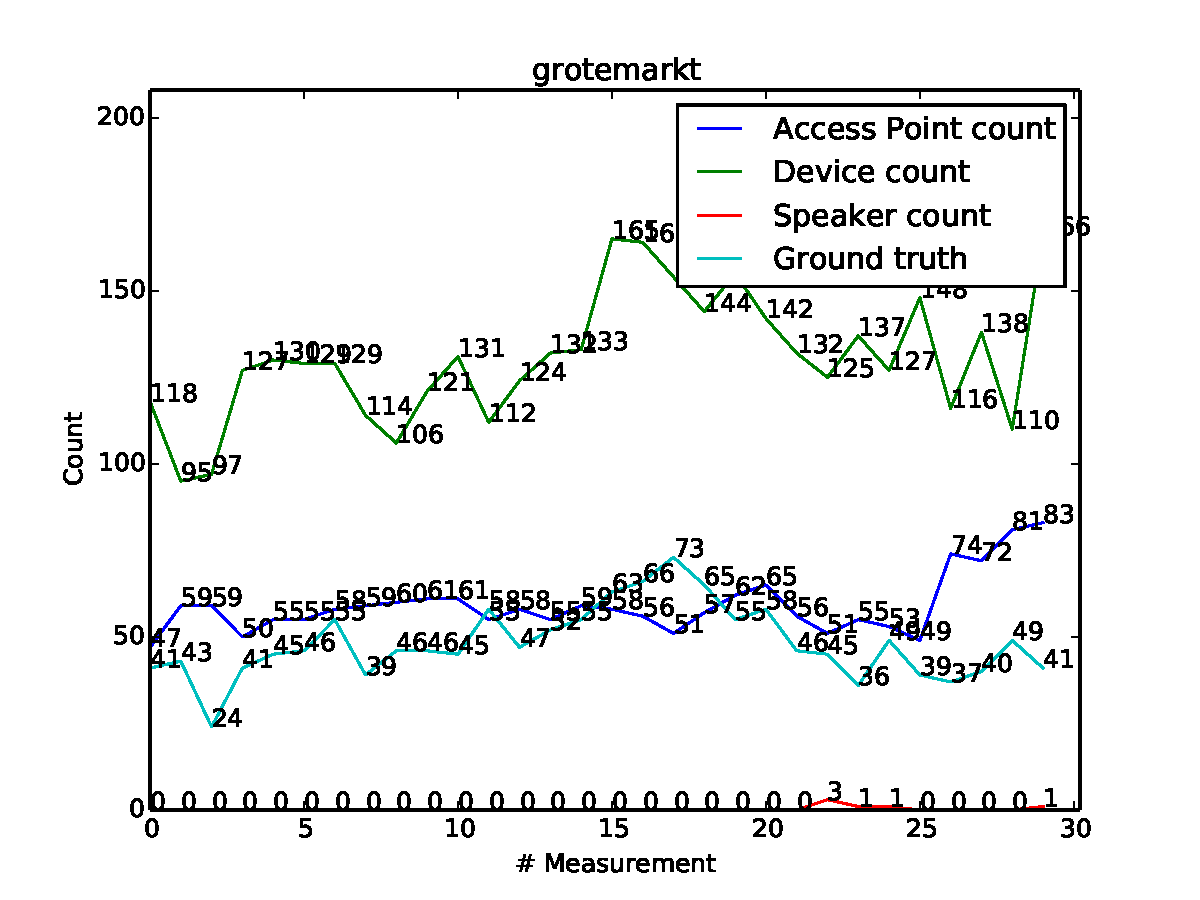
\includegraphics[width=0.7\textwidth]{./img/result/day/day2/grotemarkt-20161027}
    }
  }\\
  \subfloat[day 3]{
    \label{fig:grotemarkt-day3}{
      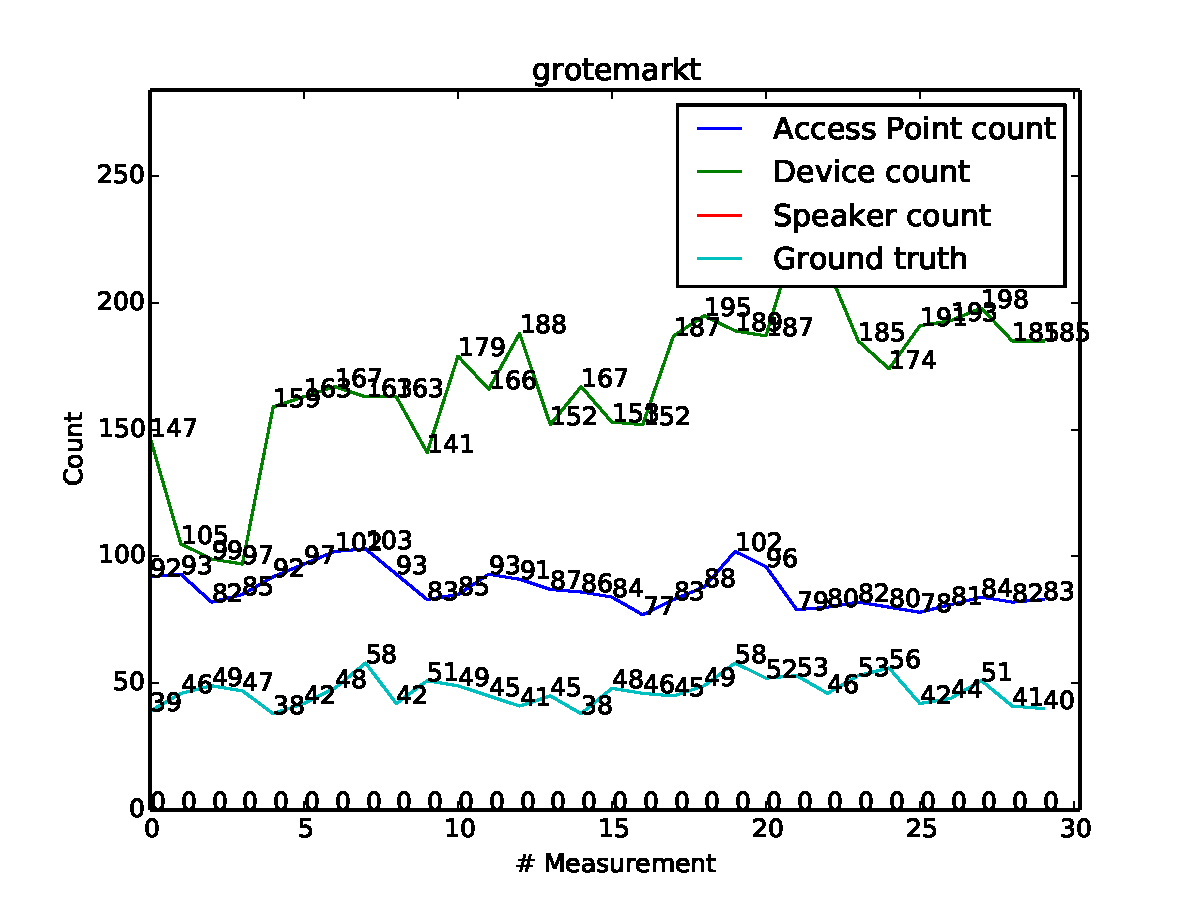
\includegraphics[width=0.7\textwidth]{./img/result/day/day3/grotemarkt-20161028}
    }
  }
  \subfloat[day 4]{
    \label{fig:grotemarkt-day4}{
      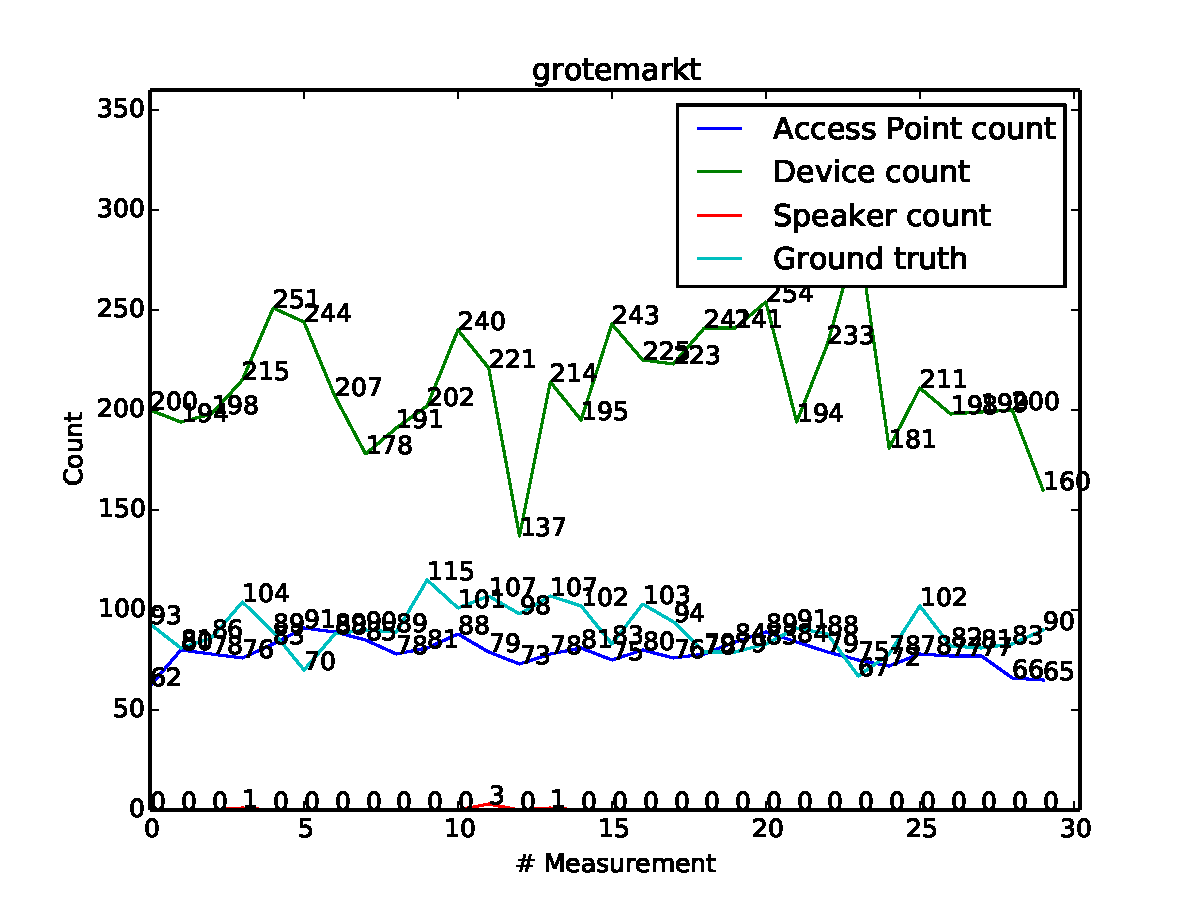
\includegraphics[width=0.7\textwidth]{./img/result/day/day4/grotemarkt-20161029}
    }
  }
  \end{adjustwidth}
  \caption[The line chart of sensor readings at Grote Markt.]
  {The line chart of sensor readings at \textit{Grote Markt} in four days of experiment.}
  \label{fig:result-grotemarkt-line-chart}
\end{figure}

